\documentclass[12pt]{article}
\usepackage[margin=1in]{geometry}
\usepackage{graphicx}
\usepackage{hyperref}
\title{LorentzTrack Particle Orbit Code}
\author{I.H.Hutchinson}
\begin{document}
\maketitle
\section{What it does}

The code LorentzTrack is a simple fortran code that solves for the
orbit of a charged particle in specified electric and magnetic fields,
using a fourth order Runge-Kutta numerical technique. It plots the
orbit in a 3-D perspective plot with simple animation. The user can
control the position of the viewer, the initial position and velocity
of the particle, and choose the field configuration from a list of
built-in cases.

\section{How to run it Precompiled on Athena Linux}

Type in to the terminal the stuff in \verb!fixed width font! below:
\begin{enumerate}
\item Log in to athena (linux). From a linux local machine
  \verb! ssh athena.dialup.mit.edu!. 
  From Windows you need something like xwin32
  installed to ssh and display the graphics.
\item \verb!add 22.611j!
\item \verb!cp -a /mit/22.611j/particle_orbits/ .! to clone the
  program and input files.
\item \verb!cd particle_orbits! enter your cloned version directory
\item \verb!./lorentztrack! to run the
  default case.
\item Watch the plot in the graphics window that will pop up.
\item To terminate, click in the graphics window.
\item To do a different case add the name of one of the input files on
  the command line after the executable. E.g.
  \verb!./lorentztrack toroidal.dat!
\end{enumerate}

\begin{figure}[htp]
  \centering
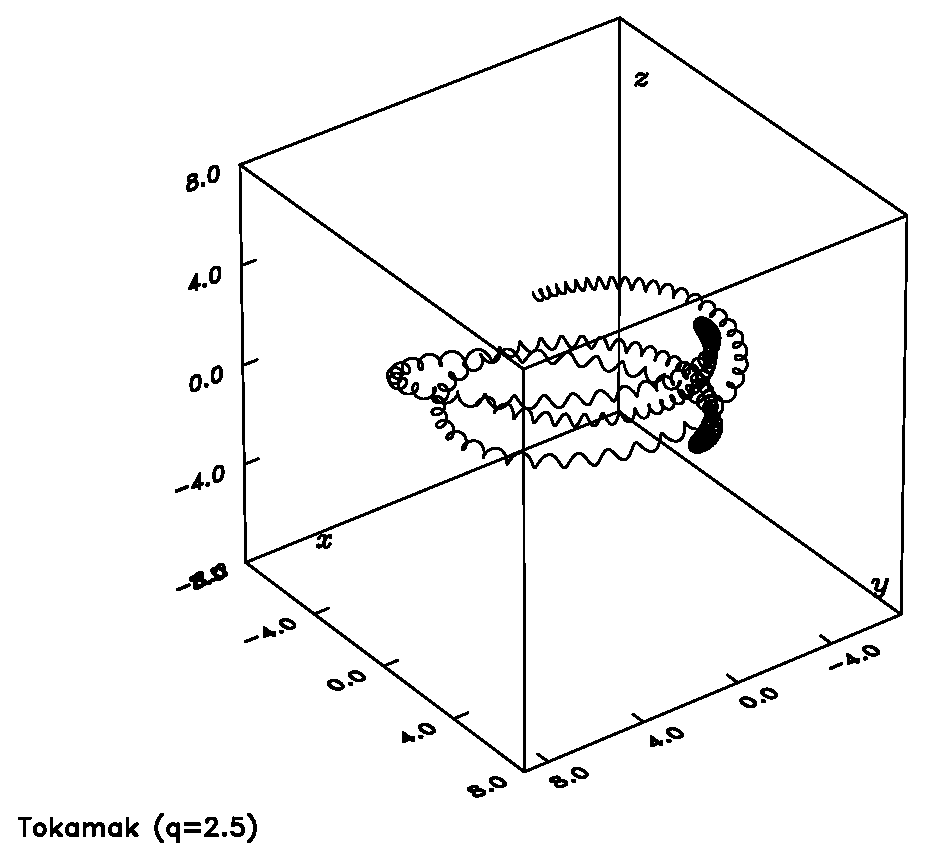
\includegraphics[width=4 truein]{toktrack}  
  \caption{Here's an example plot.}
  \label{fig:toktrack}
\end{figure}

\section{To run Precompiled on MSWindows}

Download the file \verb!lorentztrackwin.zip! to a convenient directory
on your computer. Unzip the archive to extract the archive's files
into that directory. Run the executable \verb!lorentztrack.exe!. To do
other cases, open a command line, navigate to the directory, and enter
a command like \verb!lorentztrack toroidal.dat!.


\section{Input and control files}

The data files in that directory ending with \verb!.dat! are different
examples. Use the above command line with the
name of the file which contains the case you want. They are simple
text files that can be read by any editor. The first line is a
comment/description. 

If you want to change the input parameters, edit your own copies of
the files. You should not be able to change the ones in the locker. In
addition to the first line, which is ignored by the code, there are
input numbers for the case (integer) the initial position (3 floats)
and velocity (3 floats), the step size (don't exceed 0.2) the number
of steps (integer) and the approximate time duration of the animation
(seconds, float).

If you want to change your view of the plots, hold down and drag your
mouse in the plot windown. 

\section{Equations and units}

The equation solved is the non-relativistic equation of motion for a
particle with $q/m = 1$. Typical order of magnitude of the magnetic
fields is 1, so the cyclotron frequency is thus also of order 1.
Perpendicular velocities of order 1 therefore give rise to Larmor
radii of order 1. An electric field of magnitude 1 would give a drift
velocity of magnitude $E/B = 1$. That is rather large for comfort, so
generally we'll use smaller electric fields.

The code resides in
\begin{verbatim}
/mit/22.611j/particle_orbits/lorentztrack/lorentztrack.f
\end{verbatim}
It is not terribly long (but the plotting is complicated); feel free to
\href{lorentztrack.f}{examine it} or even hack up your own version if
you like.

\end{document}




%%% Local Variables:
%%% mode: latex
%%% TeX-master: t
%%% End:
